\documentclass[conference]{IEEEtran}
\IEEEoverridecommandlockouts
% The preceding line is only needed to identify funding in the first footnote. If that is unneeded, please comment it out.
\usepackage{cite}
\usepackage{amsmath,amssymb,amsfonts}
\usepackage{algorithmic}
\usepackage{graphicx}
\usepackage{textcomp}
\usepackage{xcolor}
\usepackage{array}
\usepackage{booktabs}
\usepackage{subfigure}
\usepackage[ruled]{algorithm2e}
\usepackage{verbatim}


\def\BibTeX{{\rm B\kern-.05em{\sc i\kern-.025em b}\kern-.08em
    T\kern-.1667em\lower.7ex\hbox{E}\kern-.125emX}}
\begin{document}

\title{Deep Learning and Data Randomness based Blind Recognition of Channel Codes\\

\thanks{The work described in this paper was funded by the Hainan Province Science and Technology Special Fund (No. ZDYF2021GXJS216), the Hainan Province Major Science and Technology Project (No. ZDKJ2021052), the National Natural Science Foundation of China (No. 62162020). The authors would like to thank anonymous reviewers, Associate Editor and Editor for their constructive comments and for improving the manuscript. (\textit{Corresponding author: Chunjie Cao})}}


\author{\IEEEauthorblockN{Haifeng Peng\textsuperscript{1,2}, Chunjie Cao\textsuperscript{1,2}, Yang Sun\textsuperscript{1,2}, Haoran Li\textsuperscript{1,2}, Kangrui Ye\textsuperscript{1,2},}
\IEEEauthorblockA{
	\textsuperscript{1}School of Cyberspace Security (School of Cryptology), Hainan University, Haikou, China\\
	\textsuperscript{2}Key Laboratory of Internet Information Retrieval of Hainan Province, Hainan University, Haikou, China\\
	Email: peng\_hf@163.com, chunjie\_cao@126.com, sunydat@foxmail.com, \{flutterblu, 1660584637\}@qq.com}
}

\maketitle

\begin{abstract}
Channel coding is an efficient approach for data transmission in the wireless network, blind recognition of channel codes plays a pivotal role in non-cooperative communication and spectral scrutiny. But there are some difficulties in the low accuracy and robustness of the current research, meanwhile, most of them analyze this problem to take the coding type as the prior knowledge, which may be unknown in the actual condition. This paper proposes a multi-dimensional feature extraction algorithm, that identifies channel coding types and parameters by the neural network. A data randomness based multi-dimensional feature extraction algorithm and efficient channel attention for deep convolution neural network (ECA-Net) are used in the proposed recognizer, it had an outstanding performance in the identification of coding types, coding lengths, and coding rates. Simulation experiments showed that the proposed recognizer could realize the recognition of coding types, when the signal-to-noise ratio (SNR) is not lower than 10dB, it could achieve above 70\% of identification accuracy. On the other hand, it can improve the probability of detection by 10\% to 60\% compared with previous work for coding lengths and coding rates, which testifies the availability of this approach.


\begin{IEEEkeywords}
	Physical layer security, channel codes, blind identification, coding type.
\end{IEEEkeywords}

\end{abstract}


\section{Introduction}

\begin{figure*}[htbp]
	\centerline{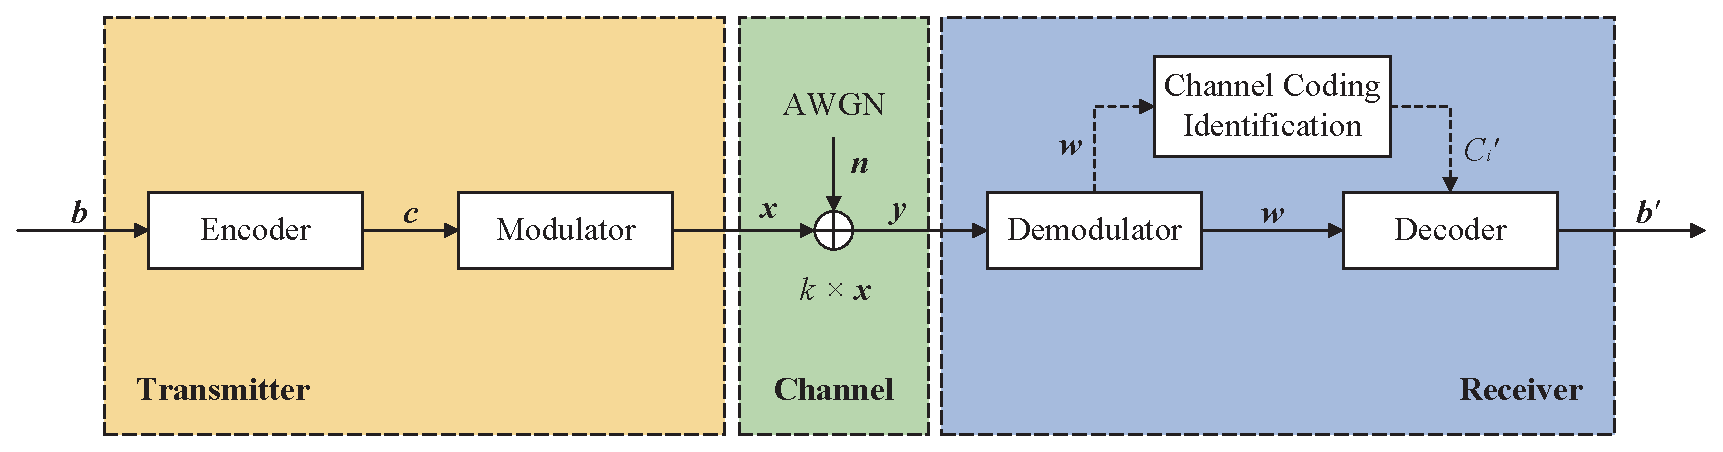
\includegraphics[scale=0.63]{figure-1-01.eps}}
	\caption{Structure of the communication link.}%	\label{fig1}
\end{figure*}

The wireless network is accessorial applied nowadays, and it causes the lack of the frequency spectrum resource \cite{wang2020high}. Arising cognitive radio alters the status quo, and remits the problem to a certain degree. Accompanying cognitive radio networks \cite{shakhov2021analysis} demands makes wireless security a key research area, such as channel codes \cite{zhang2022blind}, modulation types \cite{chu2021automatic}, medium access control (MAC) protocols \cite{gao2021mac, gao2020mac}, etc.

In cognitive radio networks, blind identification of channel codes \cite{sun2020efficient, jalali2020joint, ju2020path} is a research field to estimate the channel coding scheme of the master user, and it possesses the significance of wireless physical layer security \cite{sanchez2020physical}. Existent algorithms to distinguish channel codes need relative rich professional skills and experience, e.g., Xinyi Wang \cite{wang2020nested} et al. make use of nested construction in blind detection of polar codes by selecting the candidate of the target physical downlink control channel (PDCCH). They attempt to decode PDCCH candidates with a lower aggregation level (AL), if decoding fails, iteratively selects a higher AL to decode. But this approach to blind detection of polar codes significantly depends on the experience of the manipulator, and it needs to try to decode codewords. Although compared to exhaustive decoding reduces the number of attempts to decode, if the coding length is considerable, the computational complexity of this algorithm will increase dramatically.

Currently, most of the research about blind channel coding recognition focuses on identifying coding parameters \cite{song2021blind, liu2020blind, wu2020blind, kwon2020analysis, dean2018blind, perlstein2018fast}, i.e., coding length and rate. These researchers regard coding type as prior knowledge, still, in the factual information countermeasure and information interception scenarios, a non-cooperative transmitter may be utterly blind to a non-cooperative receiver. That is to say, the coding type of the intercepted codeword is unknown. Therefore, in addition to coding parameters, including coding lengths and rates, it is essential to consider the identification of coding types in a total blindness environment \cite{bonvard2018classification}. 

Over the last few years, the evolution of deep learning makes itself embody functionality in image classification \cite{chen2020sparsity} and natural language processing \cite{otter2020survey}, deep learning has shown excellent properties in various domains by data-driven. In the meantime, because of many data in wireless communication systems, deep learning is comprehensively used in communication territories, such as modulation recognition \cite{lin2022learning}, channel estimation \cite{hu2021semi}, and radio frequency fingerprint (RRF) identification \cite{shen2022towards}. In the field of blind channel coding recognition, Boxiao Shen et al. \cite{shen2021blind} considered distinguishing coding parameters of channel codes, based on the recurrent neural network (RNN), attention mechanism, and residual neural network (ResNet), proposed three universal channel coding recognizers. Sepehr Dehdashtian et al. \cite{dehdashtian2021deep} based on deep learning, researched blind recognition of channel codes under the AWGN channel and the Rayleigh fading channel, recovered channel coding parameters on the candidate set by the received signal. Still, there is a significant difference between the actual fading circumstance and the Rayleigh fading model \cite{besser2020reliability}.

\begin{comment}
	The travel path of electromagnetic waves in interspace is complicated and changeable, signal would suffer multi-path fading effect \cite{chen2017various, rao2011performance, makki2012arq} during transmitting procedure. Multi-path propagation and shadowing from obstacles cause fading, and it impacts the performance of wireless communication systems \cite{priyanka2018k}. Sepehr Dehdashtian et al. \cite{dehdashtian2021deep} based on deep learning, researched blind recognition of channel codes under AWGN channel and Rayleigh fading channel, and recovered channel coding parameters on the candidate set by the received signal. Still, there is a significant difference between actual fading and Rayleigh fading model \cite{rini2018capacity}. Beyond that, most research on blind recognition of channel codes has focused on the AWGN channel until now, but there are signal distortions by multi-path fading effect in actual correspondence. 
\end{comment}

In this paper, we propose a recognizer based on efficient channel attention for deep convolutional neural networks (ECA-Net) \cite{Wang_2020_CVPR}, which could blindly identify coding types, lengths, and rates using deep learning. Meanwhile, a multi-dimensional feature extraction algorithm based on data randomness \cite{liu2020security} is proposed to dispose of the received codewords, and this recognizer could distinguish channel codes in intercept codewords that are coded with different coding types and parameters. Through enough experiments, we have proved that our recognizer based on deep learning architecture could achieve high performance on blind identification of channel codes. Even without prior knowledge of coding types and parameters, i.e., this recognizer could realize completely blind identification of channel codes.


%\begin{figure}[htbp]
%	\centerline{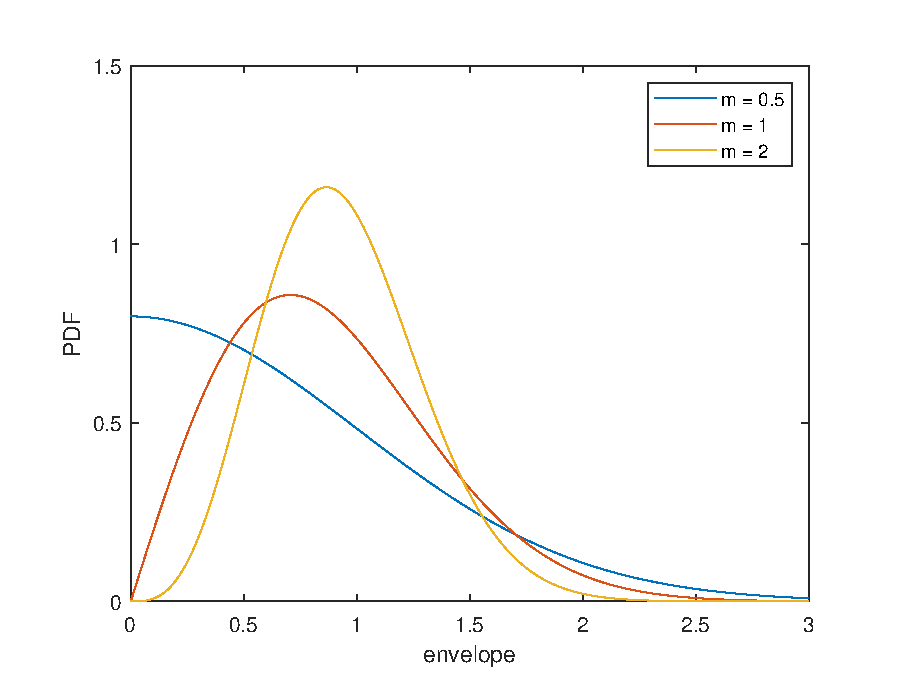
\includegraphics[scale=0.65]{figure-2.eps}}
%	\caption{PDF of the envelope at Nakagami-m fading channel.}%	\label{fig1}
%\end{figure}


The residue of this paper is organized as follows. Section II formulates the problems of channel coding recognition and explains data randomness detection. Section III discusses the proposed multi-dimensional feature extraction algorithm and the ECA-Net based recognizer for blind identification of channel codes. Section IV gives the results of simulation experiments. Section V concludes this paper.



\section{Preliminaries}

\subsection{System Structure}
In non-cooperate communications \cite{dai2019learning}, the status of the transmitter is entirely unknown to the receiver, and the receiver can only intercept signals. The goal of blind channel coding recognition is to analyze the type and parameters that the transmitter uses via the received signal. 

The communication model under fading conditions is shown in Fig. 1. An information source generates a bit information stream $\boldsymbol{b} = ({b}_{1}, {b}_{2}, \cdots, {b}_{n})$, where $n$ is the length of the bit sequence. The transmitter codes the bit information stream $\boldsymbol{b}$ using channel coding parameters $C_i$, which are from the candidate set $\Theta={C_{1}, C_{2}, \cdots, C_{N}}$, where $N$ $(1 < i < N)$ is the number of channel coding parameters in the set. Then gets the codewords $\boldsymbol{c}=({c}_{1}, {c}_{2}, \cdots, {c}_{n})$, where $c_{i} \in {GF}(2)$. Codewords would be modulated in BPSK as $\boldsymbol{x}$, which equals $\boldsymbol{c}^{BPSK}$, and transferred to the channel. The non-cooperate receiver would intercept the signals $\boldsymbol{y}$ from the channel, and it could be written as
\begin{equation}
	\boldsymbol{y} = k \times \boldsymbol{c}^{BPSK}+\boldsymbol{n},
\end{equation}
where $k$ is the loss of signal by channel fading, $\boldsymbol{c}^{BPSK} \in \{+1,-1\}$ is the modulated symbol of the codeword $\boldsymbol{c}$, and $\boldsymbol{n}$ is the zero-mean AWGN, which is independent and identically distributed with noise power $\sigma^{2}$. The received signals $\boldsymbol{y}$ go through demodulation, and become $\boldsymbol{w} = (w_{1}, w_{2}, \ldots, w_{n})$. The neural network would recognize codewords $\boldsymbol{w}$, to get the classification result with coding parameters $C_i^{\prime}$. Finally, the receiver will decode $\boldsymbol{w}$ by the identified $C_i^{\prime}$, and get the intercepted bit information $\boldsymbol{b}^{\prime}$.

In cooperative communication, the coding parameters are known by the receiver. But in non-cooperative communication, i.e. electronic warfare, the coding parameters are unknown.


\subsection{Data Randomness Test}
Data randomness occupies a very crucial position in cryptology, and the randomness of the output sequence is a significant aspect of evaluating a cryptographic algorithm. A random sequence should be able to through most of the data randomness test \cite{qu2021test}, each element of the sequence is independent and identically distributed.

Data randomness detection refer to a binary sequence, consider using a series of statistical test method to judge whether it is a really random sequence, and calculate the disparity between them. The data randomness test not only needs to consider the probability of the next bit in the sequence, but also should use some sample sequences to infer whether the sequence is reasonable.

National institute of standards and technology (NIST) \cite{lee2021nist} suggested the NIST SP800-22 criterion \cite{iwasaki2019deriving}, which is the most comprehensive data randomness test method. NIST SP800-22 criterion includes 15 test methods, each generating $P$ by the corresponding test sequence. Then designate significance level $\alpha$, the test sequence pass the test when $P \geq \alpha$, otherwise do not pass the test. In addition, to make an integrated judgment, it is requisite to select different sample sequences, that would generate different $P$. Concerning multiple sets of the tests for the different sample sequences, if the test pass rates satisfy
\begin{equation}
	r \in  \left[P^{\prime} - 3\sqrt\frac{{P^{\prime}}(1 - P^{\prime})} m, P^{\prime} + 3\sqrt\frac{{P^{\prime}}(1 - P^{\prime})} m \right],
\end{equation}
where $P^{\prime} = 1 - \alpha$, $m$ is the number of the sample sequences, i.e. the times of the tests, and it can determine that the test sequence passes the test. It can also divide the interval $[0, 1]$ into 10 sub-intervals, and calculate the number of $P$ that fall into each sub-interval, then perform the fitting calculation with
\begin{equation}
	\chi^2 =  \sum_{i=1}^{10} \frac{(n_i - \frac{m}{10})^2} {\frac{m}{10}},
\end{equation}
\begin{equation}
	P^{\prime} =  \frac{1}{\Gamma(\frac {9} {2})} \int_{0}^{x} e^{-t} t^{\frac {\chi^2} {2} - 1}\, dt,
\end{equation}
where $n_i$ is the number of $P$ that fall into the $i$-th sub-interval. Once more select another significance level $\beta$, if it satisfies $P^{\prime} \geq \beta$, it can tell $P$ obeys uniform distribution. In other words, the test sequence passes the data randomness test.

Different sequences would get different results in the data randomness test, by parity of reasoning, different channel codes with different coding parameters would also get different results. Therefore, feature vectors of channel codes could be obtained by data randomness detection, and we proposed a multi-dimensional feature extraction algorithm of channel codes based on data randomness. 

\begin{comment}

\subsection{Nakagami-m Fading}
In the transmitting procedure of electromagnetic wave, on account of reflection, refraction, diffraction, the path that signal transfer is disparate, and the signal that the receiver gets is superposed with multi-path signal, which is caused the multi-path effect. Meanwhile, there is the Doppler principle in signal transmission, it would give rise to an errand between transmitted signal frequency and received signal frequency. The research emphasis of wireless fading is the small-scale fading by multi-path effect and Doppler principle.

Nakagami-m fading \cite{le2020wireless} channel could emulate different channel fading conditions by opposite argument $m$, and the obtained data is highly identical to experimentally measured values. This model could preferably simulate components of the signal, including Gaussian, Rice, Rayleigh, etc. The theory of Nakagami-m fading with
\begin{equation}
	{R}_{Nakagami }({t}) = {a}\left|{g}_{1}({t})\right| + {b} \sqrt{{g}_{2}^{2}({t}) + {g}_{3}^{2}({t})} + {c},
\end{equation}
where $g_1(t)$, $g_2(t)$, $g_3(t)$ are standalone AWGN sequences, $a, b, c$ are undetermined coefficients, which are related to fading average power $\Omega$ and fading factor $m$. Nakagami-m fading is based on actual measured data and curve fitting, the envelope and phase of corresponding probability density function (PDF) are
\begin{equation}
	{p}({r}) = \frac{2}{\Gamma({m})}\left(\frac{m}{\Omega}\right)^{m} {r}^{2 {~m}-1} {e}^{-\frac{m}{\Omega} {r}^{2}}, {r} \geq 0,
\end{equation}
\begin{equation}
	{p}(\varphi) = \frac{\Gamma({m})|\sin 2 \varphi|^{{m}-1}}{2^{{m}} \Gamma^{2}\left(\frac{{m}}{2}\right)}, \varphi \in[0,2 \pi),
\end{equation}
where $\Gamma(m)$ is Gamma function, $\Omega$ is the second central moment, and $\Omega = E[r^2]$, it is the average power of multi-path scattering, $m$ is the fading factor, it expresses the degree of signal attenuation by multi-path effect and scattering. When $\Omega = 1$, the probability density distribution curves of Nakagami-m fading at different $m$ are shown in Fig. 2. As seen from the figure, the degree of channel fading would be more severe as $m$ decreases. 

\end{comment}

\section{Proposed Recognition Approach}

\begin{comment}

\begin{algorithm}[h]
	\caption{Constellation formation algorithm}%算法名字
	\LinesNumbered %要求显示行号
	\KwIn{Channel ouput $\boldsymbol{y}$, prior knowledge $L_a(\boldsymbol{v})$, $L_a(\boldsymbol{d})$}%输入参数
	\KwOut{Codeword sequence $\boldsymbol{w}$, prior knowledge $L_{a +   1}(\boldsymbol{v})$, $L_{a + 1}(\boldsymbol{d})$}%输出
	
	\textbf{Step 1: Demodulation module}\\ %\;用于换行
	\If{$L_a(\boldsymbol{v})$ is null}{
		Initialize $L_a(\boldsymbol{v})$\;
	}
	\For{$\boldsymbol{y}$ is not null}{
		Calculate $\boldsymbol{y}$ and $L_a(\boldsymbol{v})$\;
		Generate external knowledge $L_e(\boldsymbol{v})$\;
		Split $L_e(\boldsymbol{v})$ into $L_a(\boldsymbol{c})$ and $L_e(\boldsymbol{t}_1)$
	}
	
	\textbf{Step 2: Formation coding module}\\
	\If{$L_a(\boldsymbol{d})$ is null}{
		Initailize $L_a(\boldsymbol{d})$\;
	}
	\For{$L_a(\boldsymbol{c})$ is not null}{
		Calculate $L_a(\boldsymbol{c})$ and $L_a(\boldsymbol{d})$\;
		Generate external knowledge $L_e(\boldsymbol{c})$ and $L_e(\boldsymbol{d})$\;
		Combine $L_e(\boldsymbol{d})$ with $L_e(\boldsymbol{t}_1)$ to $L_a(\boldsymbol{u})$\;
	}
	\For{$L_a(\boldsymbol{u})$ is not null}{
		Calculate $L_a(\boldsymbol{u})$\;
		Generate codeword sequence $\boldsymbol{w}$\;
		Export external knowledge $L_e(\boldsymbol{u})$\;
		Split $L_e(\boldsymbol{u})$ into $L_{a + 1}(\boldsymbol{d})$ and $L_a(\boldsymbol{t_1})$\;
		Combine $L_a(\boldsymbol{t}_1)$ with $L_e(\boldsymbol{c})$ to $L_{a + 1}(\boldsymbol{v})$\;
	}
	
	Output $\boldsymbol{w}$, $L_{a + 1}(\boldsymbol{d})$, $L_{a + 1}(\boldsymbol{v})$\;
\end{algorithm}

\subsection{Data Preprocessing}
For solving the signal distortion by channel fading, we propose a constellation formation algorithm under Nakagami-m fading channel. Constellation formation algorithms aim to increase the probability of selecting the constellation close to the origin. We alter the likelihood of bit 0 and bit 1 in the output sequence, and use the constellation map to maximize the likelihood of bit 0.

The constellation formation algorithm that we designed could be implemented by Algorithm 1, it can be seen that the proposed constellation formation algorithm includes a demodulation module and a formation coding module. The input of this algorithm is the received signals $\boldsymbol{y}$ from the channel, the output is codewords $\boldsymbol{w}$. Prior knowledge $L_a(\boldsymbol{v})$ and $L_a(\boldsymbol{d})$ need to be initialized for the first time to run.

Demodulation module makes $\boldsymbol{y}$ and $L_a(\boldsymbol{v})$ as input, in each symbol $\boldsymbol{v}$, calculates external knowledge of each bit $v_k (k = 1, 2, \cdots, m)$, and outputs external knowledge such that
\begin{equation}
	L_{e}(v_{k}) = \ln \frac
	{\sum_{\bar{x} \in X_{k}^{0}} e^{-\frac{y - h \cdot \bar{x}} {N_{0}} + \sum_{n = 1 \atop n \neq k}^{m} f_{n}(\bar{x}) L_{a}(v_{n})}}
	{\sum_{\bar{x} \in X_{k}^{1}} e^{-\frac{y - h \cdot \bar{x}} {N_{0}} + \sum_{n = 1 \atop n \neq k}^{m} f_{n}(\bar{x}) L_{a}(v_{n})}},
\end{equation}
where $X_{k}^{0}$ is a subset of set $X$, which includes the constellation that contains the $k$-th bit $q \in \{0, 1\}$ of the constellation label, $f_{n}({x})$ is the $n$-th bit of constellation $x$, and $f_{n}({x}) = q$. The external knowledge $L_{e}(\boldsymbol{v})$ would be splitted into two information streams $L_{a}(\boldsymbol{c})$ and $L_{e}(\boldsymbol{t}_1)$. In formation coding module, information stream $L_{a}(\boldsymbol{c})$ would be calculated with prior knowledge $L_a(\boldsymbol{d})$, generate external knowledge $L_e(\boldsymbol{c})$ and $L_e(\boldsymbol{d})$, they can be given as
\begin{equation}
	L_{e}(c_{k}) = \ln \frac
	{\sum_{\bar{c} \in C_{k}^{0}} e^{\sum_{n = 1}^{K_{s}} d_{n} L_{a}(d_{n}) + \sum_{l=1 \atop l \neq k}^{N_{s}} \bar{c}_{l} L_{a}(\bar{c}_{l})}}
	{\sum_{\bar{c} \in C_{k}^{1}} e^{\sum_{n = 1}^{K_{s}} d_{n} L_{a}(d_{n}) + \sum_{l = 1 \atop l \neq k}^{N_{s}} \bar{c}_{l} L_{a}(\bar{c}_{l})}},
\end{equation}
\begin{equation}
	L_{e}(d_{k}) = \ln \frac
	{\sum_{\bar{d} \in D_{k}^{0}} e^{\sum_{l = 1 \atop l \neq k}^{K_{s}} \bar{d}_{l} L_{a}(\bar{d}_{l}) + \sum_{n = 1}^{N_{s}} c_{n} L_{a}(c_{n})}}
	{\sum_{\bar{d} \in D_{k}^{1}} e^{\sum_{l = 1 \atop l \neq k}^{K_{s}} \bar{d}_{l} L_{a}(\bar{d}_{l}) + \sum_{n = 1}^{N_{s}} c_{n} L_{a}(c_{n})}},
\end{equation}
where $C_{k}^{q}$ and $D_{k}^{q}$ are respectively the set of symbols $c$ and $d$ with the $k$-th bit $q \in  \{0, 1\}$, $c_k$ and $d_k (k = 1, 2, \cdots, K_s)$ are respectively the $k$-th bit of symbol $c$ and $d$, $c_n$ and $d_n$ are respectively the $n$-th bit of symbol $c$ and $d$, which is related to symbol $\bar{c}$ and $\bar{d}$. External knowledge $L_e(\boldsymbol{d})$ and $L_e(\boldsymbol{t}_1)$ would be combined with prior knowledge $L_a(\boldsymbol{u})$, then generate output codeword sequence $\boldsymbol{w}$ by calculation, and export external knowledge $L_e(\boldsymbol{u})$ at the same time. Later external knowledge $L_e(\boldsymbol{u})$ would be also splitted into two information streams $L_{a + 1}(\boldsymbol{d})$ and $L_{a}(\boldsymbol{t}_1)$, therein information stream $L_{a}(\boldsymbol{t}_1)$ would be combined with external knowledge $L_{e}(\boldsymbol{c})$ to prior knowledge $L_{a + 1}(\boldsymbol{v})$. It is worth nothing that prior knowledge $L_{a + 1}(\boldsymbol{v})$ and $L_{a + 1}(\boldsymbol{d})$ are the input of the next iteration.

There are altogether $2^{K_s}$ maps in the codebook, and it would make output codewords in each map to possess minimum Hamming weight. The codebook maps $K_s$ bit input codewords in all-zero to $N_s$ bit output codewords in all-zero, then increases the $K_s$ bit input codewords by 1, and map them to $N_s$ bit output codewords of Hamming weight $\omega$, which is started from 1 and takes the minimum value currently allowed. Repeat the above steps, until the number of maps in the codebook attains $|{C}_{s}|=2^{{K}_{s}}$. 

The channel capacity $C_i$ of this system could be defined as
\begin{equation}
	C_{i} = E\left[l b\left(\frac{2^{m-1} e^{\left|-\frac{(y-x)^{2}}{2 \delta^{2}}\right|}}{\sum_{s \in X} {Pr}(s) e^{\left|-\frac{(r-s)}{2 \delta^{2}}\right|}}\right)\right],
\end{equation}
where ${E}[\cdot]$ is the expect function, ${Pr}(s)$ is the probability of forming bit, which corresponds the constellation points in planisphere. When the first bit of constellation point in planisphere is 0, make ${Pr}(s) = p_0$, relatively ${Pr}(s) = p_1$ when the bit is 1. In a system without constellation formation, $p_0 = p_1$, and denotes SNR of this time as $\text{SNR}_0$, when adding the constellation formation to the system, ${p}_{0} \neq {p}_{1}$, and denotes SNR which could reach the same capacity as $\text{SNR}_1$. In this moment $\text{SNR}_1 < \text{SNR}_0$, the gain of constellation formation algorithm could attain $(\text{SNR}_0 - \text{SNR}_1)$dB.

\end{comment}

\begin{figure}[tbp]
	\centerline{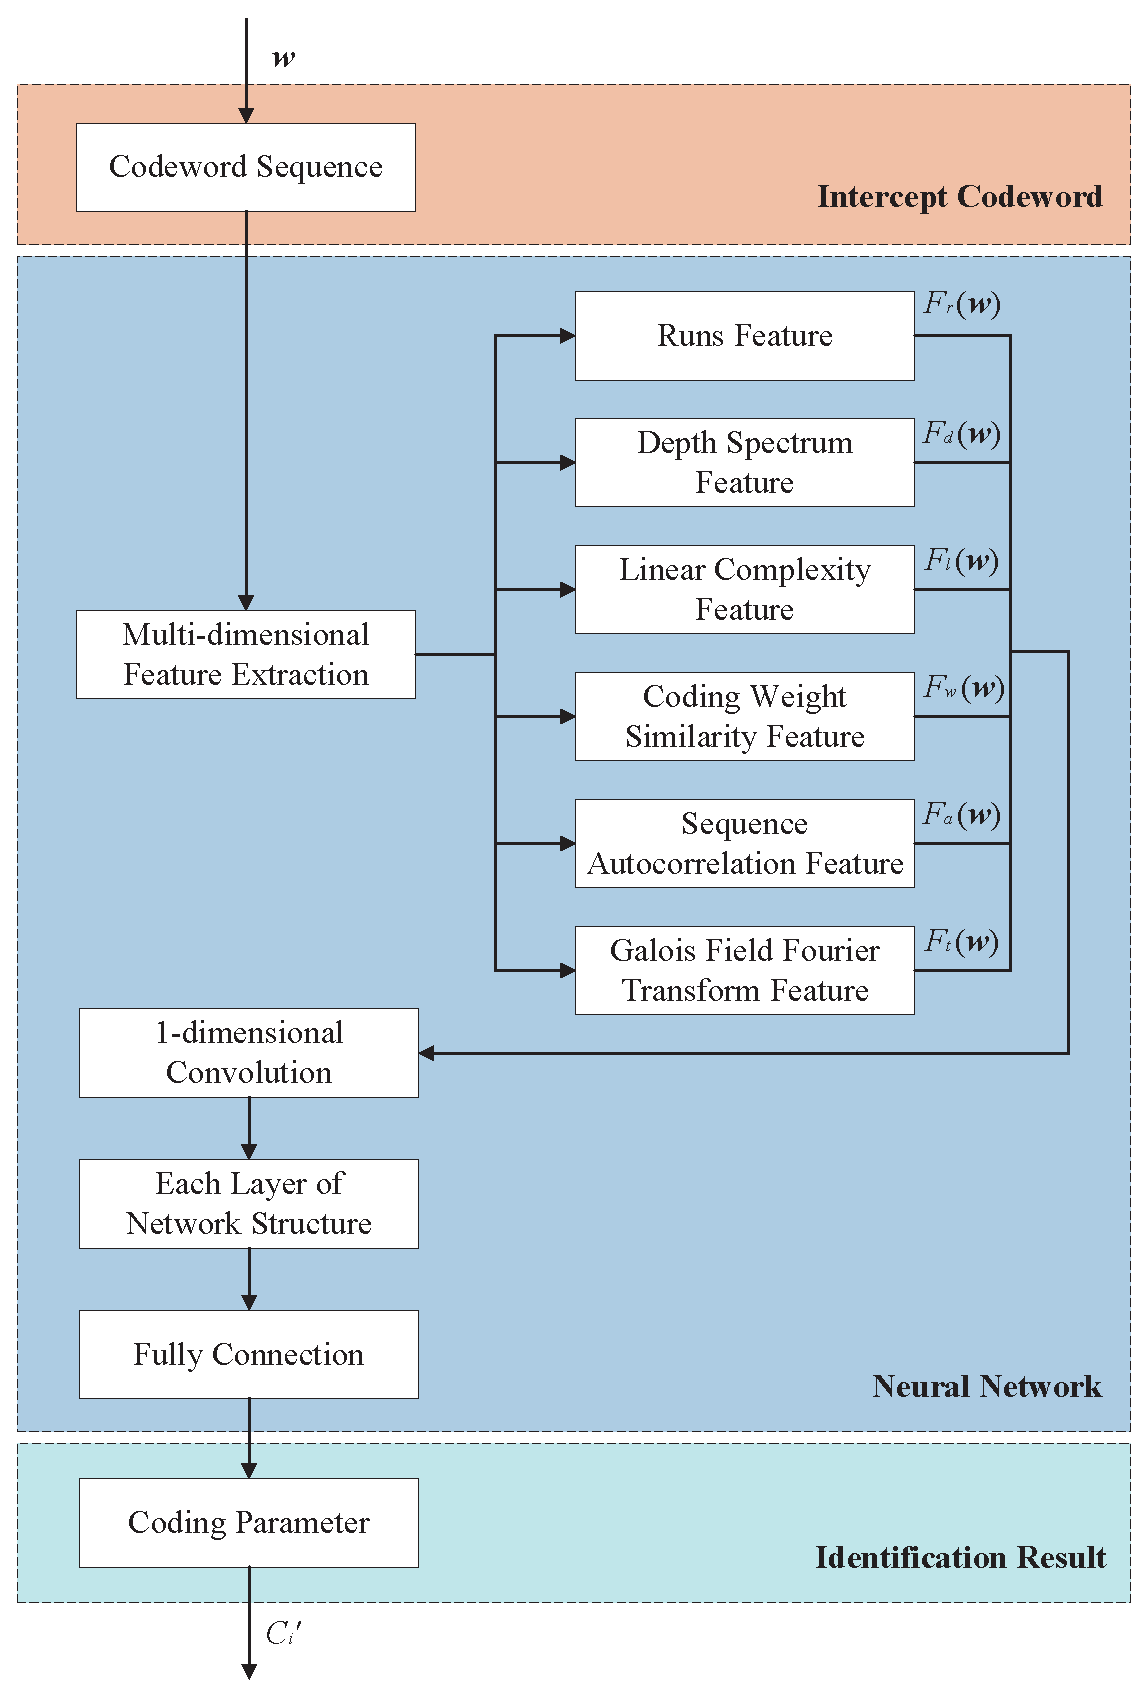
\includegraphics[scale=0.45]{figure-4-01.eps}}
	\caption{Scheme of channel coding identification.}%	\label{fig1}
\end{figure}

\subsection{Data Preprocessing}
Galois field is the essential theoretical basis of channel codes, and the intercept codewords can be seen as an $N \times K$ matrix, where $N$ is the number of frames, and $K$ is the length of the frame, it should note that $N$ and $K$ are both unknown parameters. The matrix can rearrange to a code stream, and based on Galois field $GF(p^n)$, we can get $p =$ 2 of the code stream. Then we can fill the code stream with 0, until the length of it satisfy
\begin{equation}
	(p^n - 1) \cdot n > N \cdot K,
\end{equation}
where $(p^n - 1) \cdot n$ is the length of the coding stream after filling, $p^n$ is the number of elements in Galois field $GF(p^n)$, $n$ is the minimum positive integer that makes the above formula true, and $p = 2$ in a binary sequence. The coding steam can arrange to $(p^n - 1) \times n$ matrix after filling, each of these rows with the length $n$ is a coding block, and every coding block obeys Galois field $GF(p^n)$.


\subsection{Feature Extraction}
The multi-dimensional feature extraction algorithm that we proposed is shown in Fig. 2. The intercepted codewords will feed into the neural network, and the first layer of the neural network is the multi-dimensional feature extraction algorithm based on data randomness. Then the eigenvectors would be handled with the other layers of the neural network, output the coding parameters by identification.

The number of transformations for consecutive bits 0 and 1 is differs in various binary sequences, and the number of transformations is run. Calculate the sum of the runs in the entire codeword under test is the emphasis of the runs test, and the runs are defined as
\begin{equation}
	R_{j} = \sum_{i=1}^{n-1} r_i + 1,
\end{equation}
where $j$ $(0 < j < p^n)$ is the index of the coding block, $n$ is the length of codeword $\boldsymbol{w}$, $r_i$ is 0 when bit $w_i$ equals bit $w_{i + 1}$, and is 1 when bit $w_i$ is not equivalent to bit $w_{i + 1}$,  bit $w_i$ and $w_{i + 1}$ is the $i$-th and $(i + 1)$-th bit in codeword $w$. Then can obtain the feature of runs $F_r(\boldsymbol{w}) = (R_1, R_2, \cdots, R_{p^n - 1})$. 

Depth spectrum is the feature that is generated in codeword by differential operation, and the differential operation could be operated as
\begin{equation}
	f(\boldsymbol{w}) = (w_{1} \oplus w_{2}, w_{2} \oplus w_{3}, \cdots, w_{n - 1} \oplus w_{n}),
\end{equation}
where the differential is xor to adjacent bits in binary codes. It would keep differential operation until there are all-zero results, and the differential time $d$ is codeword depth. The multiple differentials could be formulated as
\begin{equation}
	f^{d}(\boldsymbol{w}) = [0^{n-d}],
\end{equation}
where $d$ is the differential times, the minimum $d$ that can make the above equation true is the codeword depth. The codeword depth belongs to a codeword, and the depth spectrum could embody the probability of codeword depth in disparate coding parameters. The codeword depth of the $j$-th coding block can be expressed as $d_j$, and the feature of the depth spectrum can be given as $F_d(\boldsymbol{w}) = (d_1, d_2, \cdots, d_{p^n - 1})$.

It is similar to random sequences, channel codes are generated by linear feedback shift register (LFSR) in normal circumstances, so the linear complexity can be determined by calculating the length of LSFR. The coding block to be calculated can be expressed as $\boldsymbol{a} = (a_1, a_2, \cdots, a_{n})$, initialize $i = 0$, $f_0(x) = 1$, $l_0 = 0$, iterative compute $d_i = f_i(x)a_i$. When $d_i = 0$, make $f_{i + 1}(x) = f_i(x)$, $l_{i + 1} = l_i$, and $i++$ if $i < n$. When $d_i = 0$ and $l_k= 0$ $(0 \leq k \leq i)$, make $f_{i + 1}(x) = x^{i + 1} + 1$, $l_{i + 1} = i + 1$, it is similar that $i++$ if $i < n$. When $d_i = 0$ and $l_k < l_{k + 1}$ $(0 \leq k \leq i - 1)$, make $f_{i + 1}(x) = f_i(x) + x^{i - k}f_j(x)$, $l_{i + 1} = max(l_i, i - l_i + 1)$, this moment $i$ is not changing. 

After iterative calculation, the linear complexity $L$ of the coding block can be obtained, and the theoretical expectation of a random sequence can be calculated as
\begin{equation}
	\mu =  \frac n 2 + \frac {9 + (-1)^{n + 1}} {36} - \frac {\frac n 3 + \frac 2 9} {2^n},
\end{equation}
where $n$ is the length of the coding block $\boldsymbol{a}$. Then compared with the theoretical expectation $\mu$ of a random sequence, and the result is
\begin{equation}
	T_j =  (-1)^n(L_j - \mu),
\end{equation}
where $L_j$ is the corresponding linear complexity for each coding block $\boldsymbol{a}_j$, and the feature of linear complexity can be given as $F_l(\boldsymbol{w}) = (T_1, T_2, \cdots, T_{p^n - 1})$.

The information section has a constrained relationship with the parity section in the codeword, and the probability of bits in the random sequence is uniform, so there is a big difference in the coding weight distribution between the codeword and the random sequence. Calculate the probability distribution $\boldsymbol{x} = (x_0, x_1, \cdots, x_n)$ of Hamming coding weight for a coding block, the element of $\boldsymbol{x}$ represents the occurrence probability of the coding weight, and it is similar to calculating the probability distribution $\boldsymbol{y} = (y_0, y_1, \cdots, y_n)$ of Hamming coding weight for a random sequence. The variance and the covariance of coding weight probability distribution in a codeword and a random sequence such that
\begin{equation}
	D(x) = \frac{1}{n + 1} \sum_{i = 0}^{n}\left(x_i-\frac{1}{n + 1}\right)^{2},
\end{equation}
\begin{equation}
	D(y) = \frac{1}{n + 1} \sum_{i = 0}^{n}\left(y_i-\frac{1}{n + 1}\right)^{2},
\end{equation}
\begin{equation}
		COV(x, y) = \sum_{i = 0}^{n}\left(x_i - \frac{1}{n + 1}\right)\left(y_i - \frac{1}{n + 1}\right),
\end{equation}
where $x_i$ is the $i$-th element in code weight $\boldsymbol{x}$ of the coding block, and $y_i$ is the $i$-th element in code weight $\boldsymbol{y}$ of the random sequence. The probability distributions of the two vectors are statistically similar, and the coding weight similarity is
\begin{equation}
	W_j = \left[\frac{COV(x, y)}{\sqrt{D(x)} \cdot \sqrt{D(y)}}\right]^2,
\end{equation}
the discrepancy of code weight probability distribution in a codeword and a random sequence could reflect their similarity. Hence the feature of coding weight similarity can be given as $F_w(\boldsymbol{w}) = (W_1, W_2, \cdots, W_{p^n - 1})$.

The sequence autocorrelation features are based on the relationship between symbols, which is realized by the test of random sequences. The number of different elements in the original sequence and the shifted sequences with
\begin{equation}
	E_j = \sum_{i = 0}^{n - k + 1} w_{i} \oplus w_{i + k},
\end{equation}
where $k$ is logical shift delay. Shift xor addition is used to calculate the self-correlation feature, and then the feature of sequence autocorrelation can be given as $F_s(\boldsymbol{w}) = (E_1, E_2, \cdots, E_{p^n - 1})$.

Taking Galois field Fourier transform (GFFT) \cite{lin2020scheme} of the coding block can get the distribution of the spectral peak, thus detecting the periodic characteristic of the coding block, and it could be seen that the degree of deviation. GFFT is a discrete Fourier transform (DFT) \cite{chen2019new} of a coding block $\boldsymbol{a}$ in the Galois field, and DFT could be defined as
\begin{equation}
	f_j = \sum_{k = 1}^{n} a_k \left[cos\left(\frac {2\pi kj} n\right) + sin\left(\frac {2\pi kj} n\right)i \right],
\end{equation}
where $i = \sqrt{-1}$, $j \in [0, n - 1]$. The coding block is subjected to Galois field $GF(p^n)$, the GFFT matrix $\boldsymbol{M}$ can be solved first, and it is a $(p^n - 1) \times (p^n - 1)$ matrix. The coding stream after the arrangement is a $(p^n - 1) \times n$ matrix, and converts the $1 \times n$ row vector to a decimal number, get the $(p^n - 1) \times 1$ column vector $\boldsymbol{c}$. Then calculate the eigenvector of GFFT, and it can be given as
\begin{equation}
	F_g(\boldsymbol{w}) = \boldsymbol{M} \cdot \boldsymbol{c}
\end{equation}
and it is also a vector of length $(p^n - 1)$.

The features of runs, depth spectrum, linear complexity, coding weight similarity, sequence autocorrelation, and GFFT joint into a 6-dimensional eigenvector with length $p^n - 1$. It is worth noting that the GFFT feature includes the real and imaginary parts, and then the neural network would be trained and classified by the eigenvectors.


\subsection{Deep Learning Framework}
Deep learning \cite{liao2021statistical} is a significant breakthrough in computer science, and plays a central role in most computer vision systems. In recent years, deep learning is also being applied to other areas, and some encouraging results have been achieved. 

The neural network filter convolutes eigenmatrix, generates feature maps, then performs max pooling to each feature map, and records the most significant number in each feature map. In the penultimate floor, neural network joints eigenvalue to the eigenvector, finally inputs eigenvector to softmax function, and classifies data by it.

 In region size $h$, there is a filter with weight matrix $\omega$, and $h \times d$ parameters need to be estimated by $\omega$. Eigenmatrix could be denoted as $\boldsymbol{A} \in \mathbb{R}^{s \times d}$, the sub-matrix from $p$-th row to $q$-th row in eigenmatrix $\boldsymbol{A}$ is $\boldsymbol{A}[p : q]$. By repeated applying the filter to the sub-matrix in $\boldsymbol{A}$, the output $\boldsymbol{o} \in \mathbb{R}^{s - h + 1}$ from the convolution operator could be obtained, and it could be formulated as
\begin{equation}
	o_{p}=\omega * \boldsymbol{A}[{p}: {p}+{h}-1],
\end{equation}
where $p$ $(1 \leq {p} \leq {s} - {h} + 1)$ is the row in $\boldsymbol{A}$. So feature mapping $\boldsymbol{z}$ of this filter could be operated as
\begin{equation}
	\boldsymbol{z}=f(\boldsymbol{o}+\boldsymbol{b}),
\end{equation}
where $f$ is the activate function, and $\boldsymbol{b}$ is the offset item. The neural network can use filters with identical or different area sizes to learn complementary features from the input eigenmatrix, and achieve the purpose of training.


\begin{figure}[tbp]
	\centerline{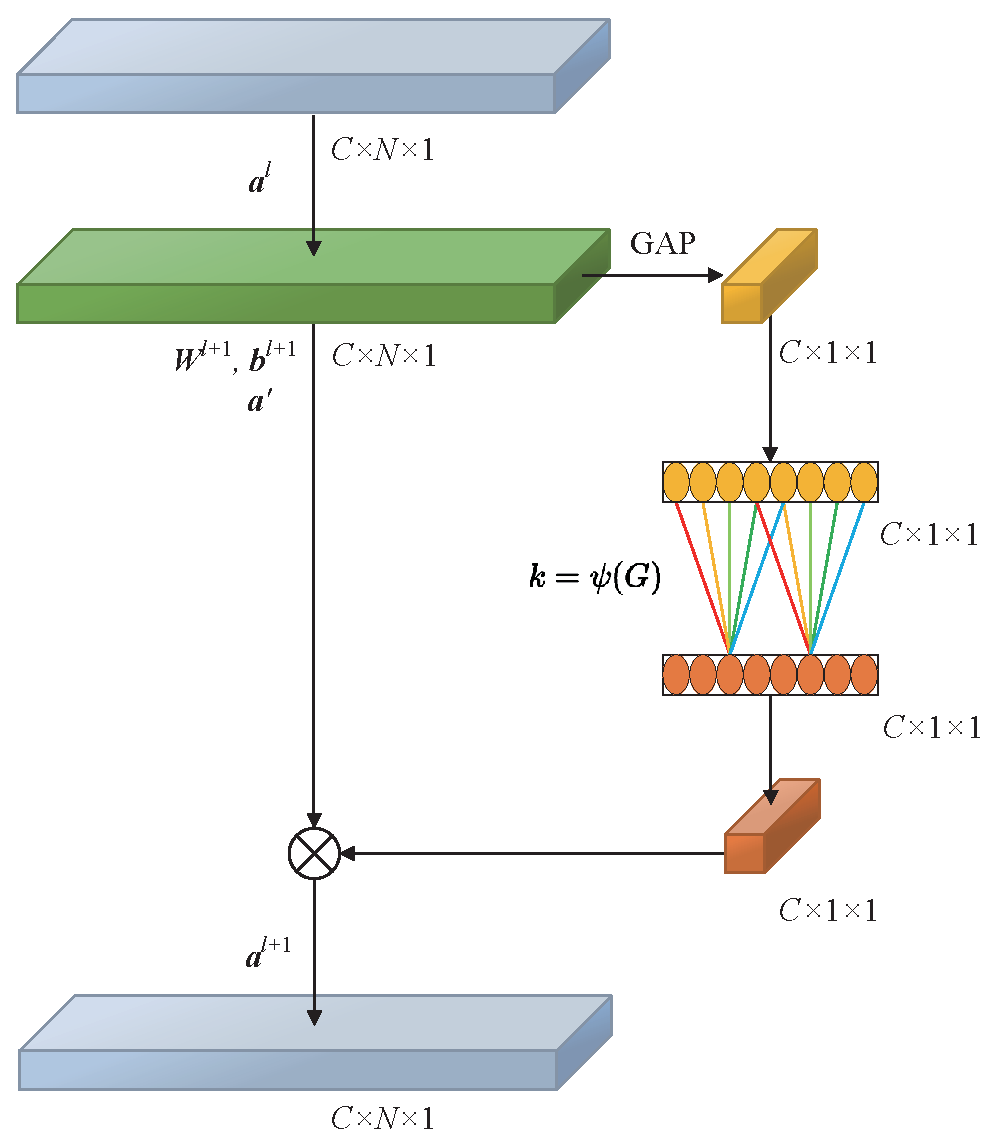
\includegraphics[scale=0.5]{figure-3-01.eps}}
	\caption{Operating principle of ECA module.}%	\label{fig1}
\end{figure}

\subsection{ECA-Net}
ECA-Net is a sort of convolutional neural network (CNN) \cite{zhang2021fast} with novel channel attention mechanisms, and it improves channel attention module based on squeeze-and-excitation network (SeNet) \cite{hu2018squeeze}. ECA-Net realized a new approach to the adaptive selection of convolutional kernel and local cross-channel interaction policy, it not only boosts the performance of complex attention modules, but also reduces the complexity of the neural network model. 

In the ECA module, the operating principle of the channel attention mechanism is shown in Fig. 3. Firstly input the features of original data, proceed with global average pooling (GAP) \cite{wang2020deep} to the features, and obtain features without dimension reduction. On this basis, the ECA module gets local cross-channel interactions by fast 1-dimensional convolution with size $k$, and parameter $k$ could be generated by adaptive function with size $C$, which is the size of the input channel. Later, using the sigmoid function, calculates the weight in each channel, and obtains features with channel attention by combining original input features and channel weights. The neural network that takes in the ECA module could extract discriminant features more efficiently, and achieve better performance based on channel dimension.

We establish ECA-Net based on ResNet \cite{wen2020transfer}, input features $X$ and convolution features $F(X)$ directly correspond to the addition of dimensions, i.e., $F(X) + X$. It avoids the gradient dissipation problem that the depth of the neural network is too deep, making the performance of the global neural network would not have to deviate as the depth increases. In residual base block, the neural network cuts in the ECA module after the third convolution, and the preponderance of channel attention mechanism perfects ResNet. It makes the neural network focus on discriminant regions of data, thus improving the performance of the neural network.


\begin{table}[tbp]
	\caption{Hyper-Parameter Selectings.}
	\begin{center}
		\begin{tabular}{cc}
			\hline
			\specialrule{0em}{3pt}{3pt}
			Description & Values \\ 
			\specialrule{0em}{2pt}{2pt}
			\hline
			\specialrule{0em}{3pt}{3pt}
			Activation & ReLU \\
			\specialrule{0em}{1pt}{1pt}
			\specialrule{0em}{2pt}{2pt}
			Optimizer & Adam \\
			\specialrule{0em}{1pt}{1pt}
			\specialrule{0em}{2pt}{2pt}
			Learning rate & 0.01 \\
			\specialrule{0em}{1pt}{1pt}
			\specialrule{0em}{2pt}{2pt}
			Batch size & 256 \\
			\specialrule{0em}{1pt}{1pt}
			\specialrule{0em}{2pt}{2pt}
			Number of iterations & 20000 \\
			\specialrule{0em}{2pt}{2pt}
			\hline
		\end{tabular}
		\label{tab1e}
	\end{center}
\end{table}


Overall models of the neural network all use cross entropy as the loss function, and the loss function of each branch could write as
\begin{equation}
	{L}_{raw} = -\log \left({P}_{r}({c})\right),
\end{equation}
\begin{equation}
	{L}_{object} = -\log \left({P}_{o}({c})\right),
\end{equation}
\begin{equation}
	{L}_{part} = -\sum_{n=0}^{N-1} \log \left(P_{p(n)}(c)\right),
\end{equation}
where $L_{raw}$, $L_{object}$, $L_{part}$ are respectively the loss functions of each branch in raw codewords, object-level codeword, part-level codeword, $c$ is the actual label of input codeword, $P_r(\cdot)$, $P_o(\cdot)$ are respectively classification probability values that softmax function takes raw codeword, object level-codeword after training by the neural network, $P_{p(n)}(\cdot)$ is the classification that softmax function takes the $n$-th codeword in part level codewords after training by the neural network, and $N$ is the number of part-level codewords. The loss function of overall neural network $L_{total}$ is defined as
\begin{equation}
	L_{total}=L_{raw}+L_{object}+L_{part},
\end{equation}
in the base of $L_{total}$, the model makes overall neural network train fitting by constantly training to optimize.


\begin{figure}[tbp]
	\centerline{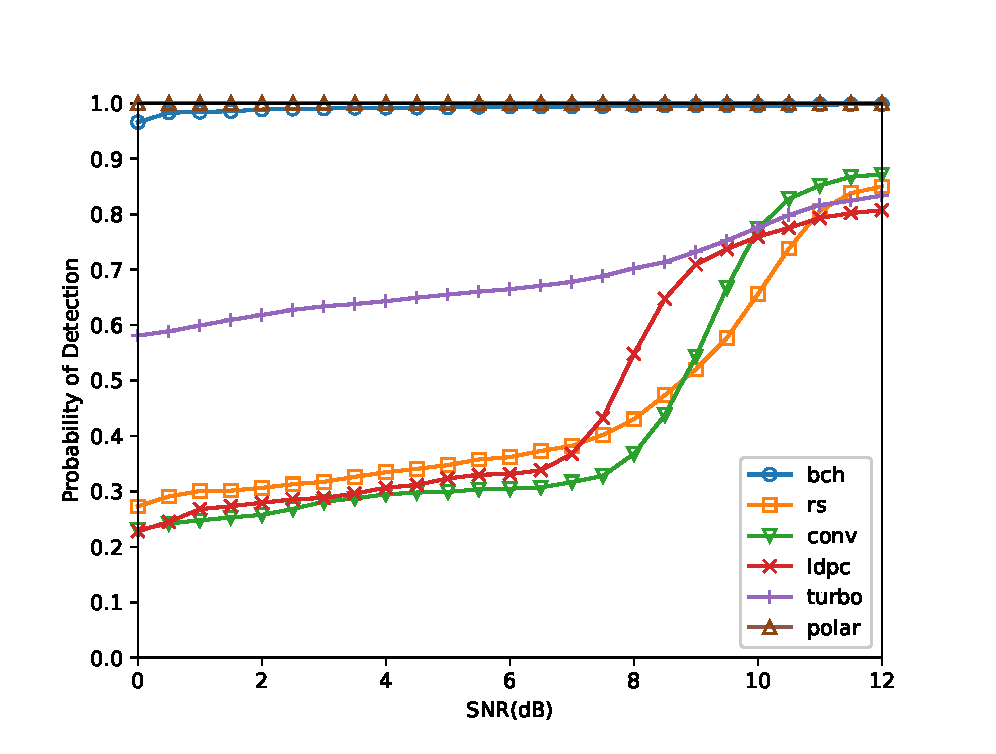
\includegraphics[scale=0.6]{result-type.eps}}
	\caption{Probability of detection among different coding types.}%	\label{fig1}
\end{figure}

\subsection{Hyper-Parameter Selection}
Hyper-parameter adjustment is the essential step in deep learning, and we select the optimal hyper-parameters after multiple experimental adjustments. To choose the best hyper-parameter, we conducted the gird search in the range of 3 to 9 for the number of residual modules, 64 to 256 for the number of convolutional kernels, 2 to 9 for the size of convolutional kernels, 0.1 to 0.001 for the learning rate, 64 to 256 for the batch size.

The number of residual modules is selected as 4, in coding type recognition, the number of convolution kernel is 64, with the sizes of 3, 5, 5, 7, and in coding parameter recognition,  the number of convolution kernel is 32, with the sizes of 3, 3, 3, 3. The softmax function on the last floor, and the training hyper-parameters in the neural network are given in Table I.

Based on the parameters in Table I, we could train a neural network model, and measure the accuracy of the trained model in blind channel coding identification. 

\begin{comment}

\begin{figure*}[htbp]
	\centerline{
		\rotatebox{0}{\scriptsize{
				~~~~~~~~~~~~
				\textbf{(a)AWGN}
				~~~~~~~~~~~~~~~~~~~~~~~~~~~~~~~~~~~~~}}
		\rotatebox{0}{\scriptsize{
				~~~~~~~~
				\textbf{(b)Rayleigh Fading}
				~~~~~~~~~~~~~~~~~~~~~~~~~~~~~~~~~~~}}
		\rotatebox{0}{\scriptsize{
				~~
				\textbf{(c)Nakagami-m Fading}
				~~~~~~~~~~~}}
	}
	\centerline{
		\subfigure{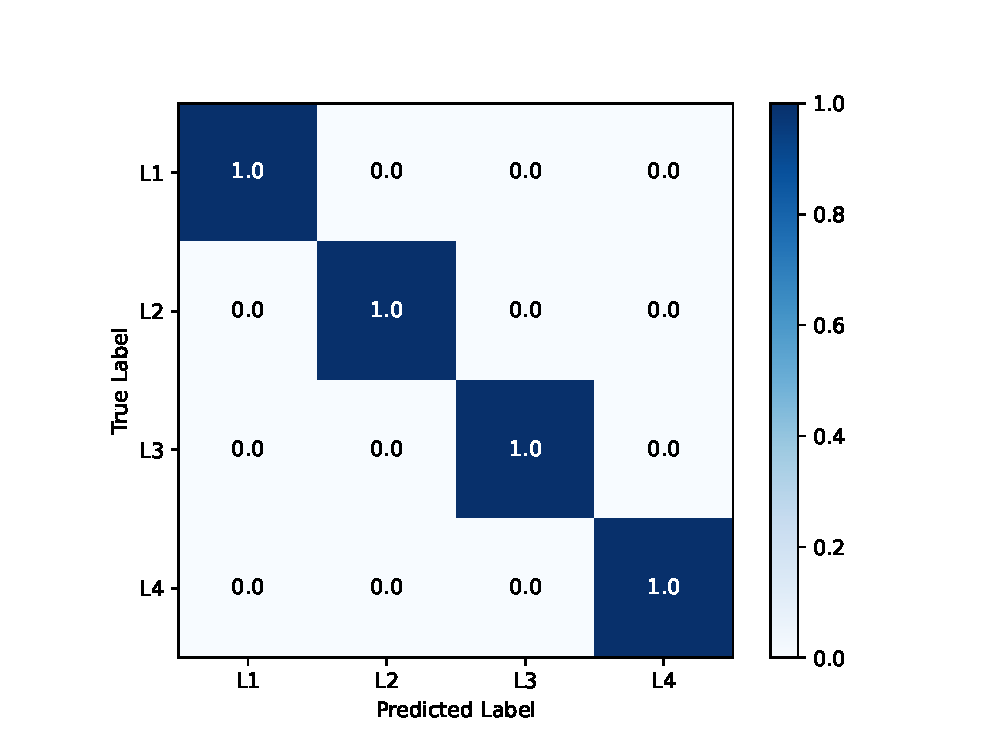
\includegraphics[scale=0.35]{confusion-1.eps}}
		\subfigure{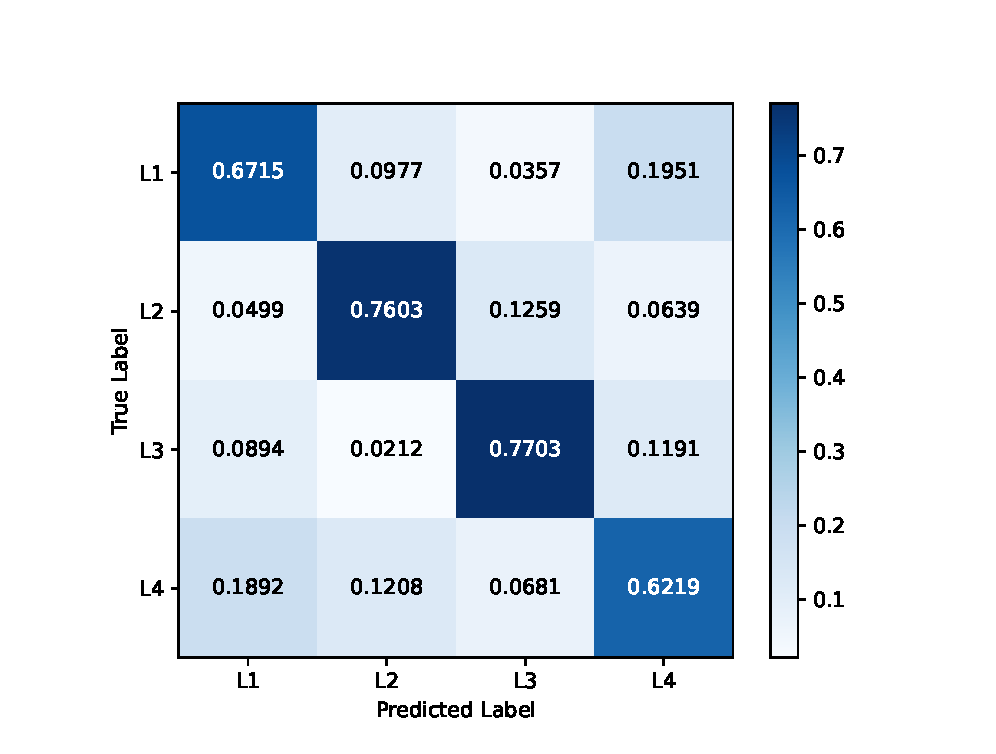
\includegraphics[scale=0.35]{confusion-2.eps}}
		\subfigure{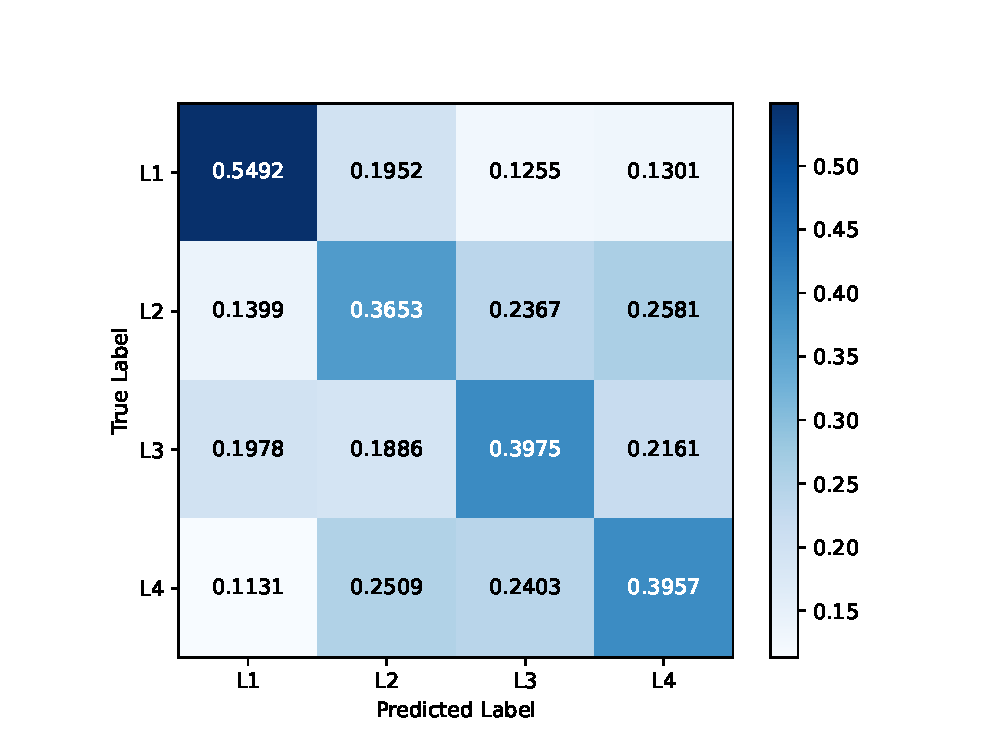
\includegraphics[scale=0.35]{confusion-3.eps}}
	}
	\caption{Confusion matrix for blind recognition of LDPC codes in different (a) AWGN channels, (b) Rayleigh fading channels, (c) Nakagami-m fading channels, at SNR 10dB.}
	\label{fig}
\end{figure*}

\end{comment}

\begin{figure}[htbp]
	\centerline{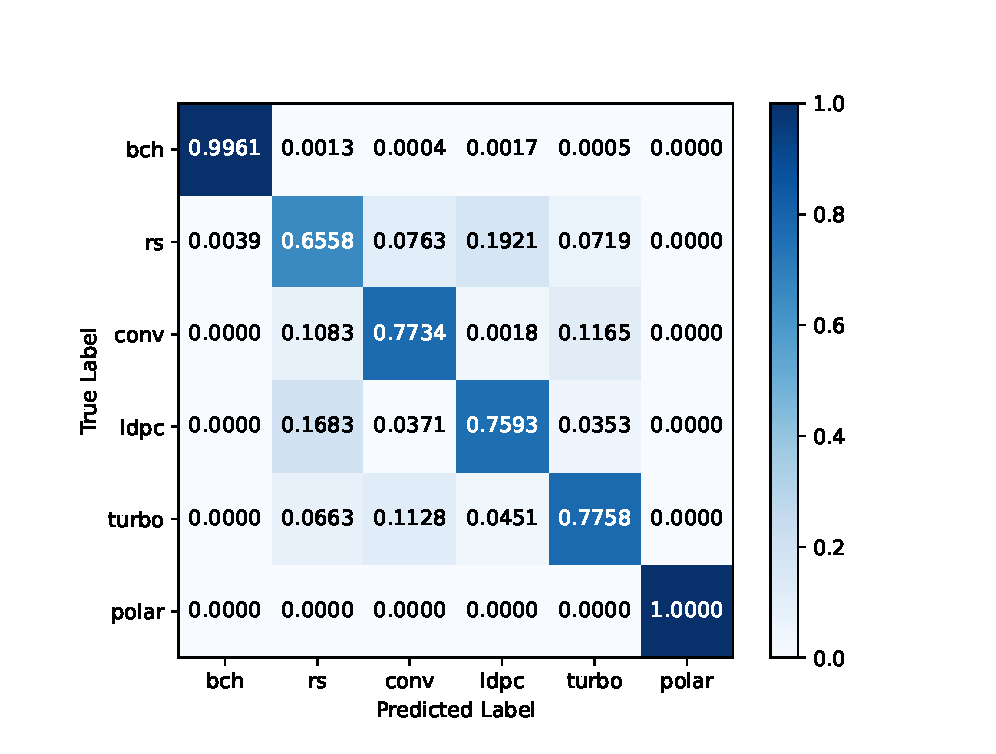
\includegraphics[scale=0.6]{confusion-type.eps}}
	\caption{Confusion matrix for coding types recognition, SNR = 10dB}%	\label{fig1}
\end{figure}

\section{Performance Emulation}
The data set we use is from \cite{shen2021blind}, and we consider identification of coding type, coding length, and coding rate in the experiments. In each module of the experiments, the numbers of the codewords in training datasets, validation datasets, test datasets are 1,200,000, 400,000, 400,000, and the range of SNR is from 0dB to 12dB in the circularly symmetric complex Gaussian noise (CSCG) channel.

We employ Windows Server 2019, Intel Xeon Gold 5117, and Nvidia RTX 2080Ti in experiments, and the experiment environment is CUDA 11.6.0, python 3.7.9, and torch 1.8.1, which is in accord with the requirement of many experiments. Because the received codewords are suffered from channel interference, including noise and fading, it would be dealt with the feature extraction algorithm at first, then identify the coding parameters $C_i^{\prime}$ by the neural network.

\begin{figure*}[tbp]
	\centerline{
		\rotatebox{0}{\scriptsize{
				~~~~~~~~~~~~
				\textbf{(1) NCD}
				~~~~~~~~~~~~~~~~~~~~~~~~~~~~~~~~~~~~~~~~~}}
		\rotatebox{0}{\scriptsize{
				~~~~~~~~
				\textbf{(2) 5-dimensional}
				~~~~~~~~~~~~~~~~~~~~~~~~~~~~~~~~~~~~~~~~~~~}}
		\rotatebox{0}{\scriptsize{
				\textbf{(3) 6-dimensional}
				~~~}}
	}
	\centerline{
		\subfigure{
			\rotatebox{90}{\scriptsize{~~~~~~~~~~~~~~~~~~~\textbf{(a) RCPC}}}
			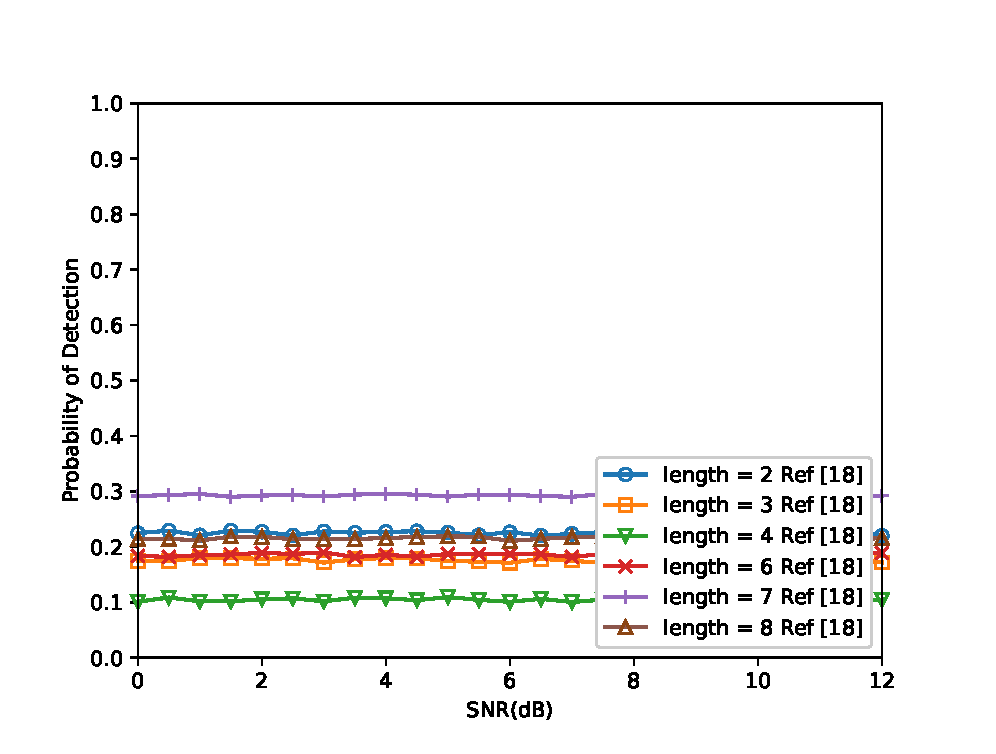
\includegraphics[scale=0.35]{result-length-conv-ncd.eps}
		}
		\subfigure{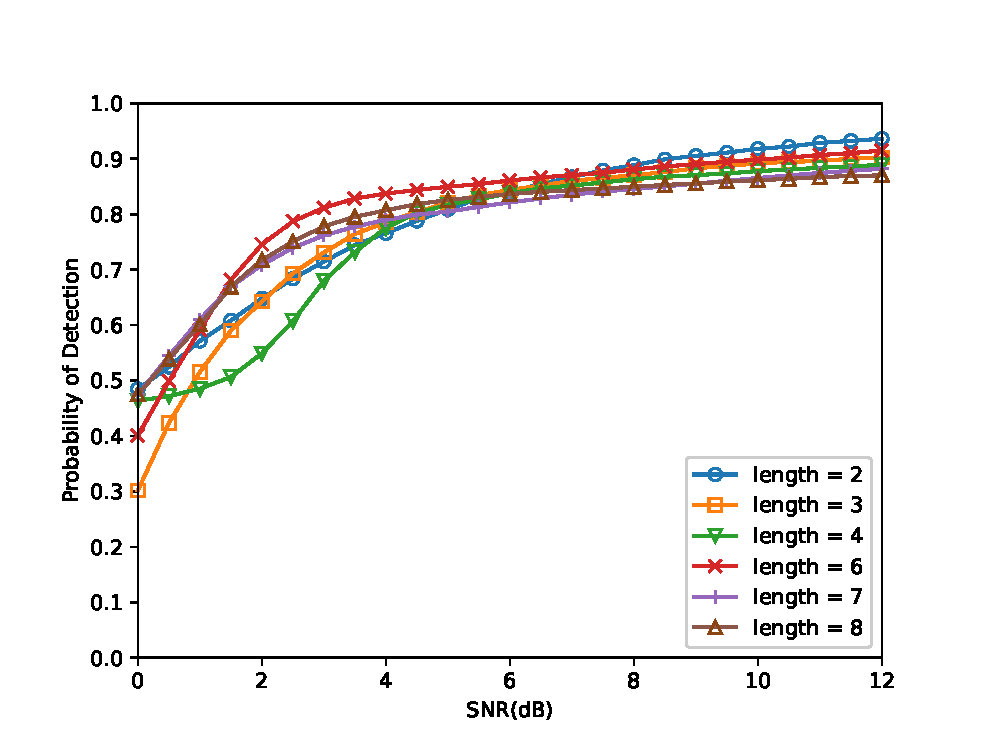
\includegraphics[scale=0.35]{result-length-conv-5.eps}}
		\subfigure{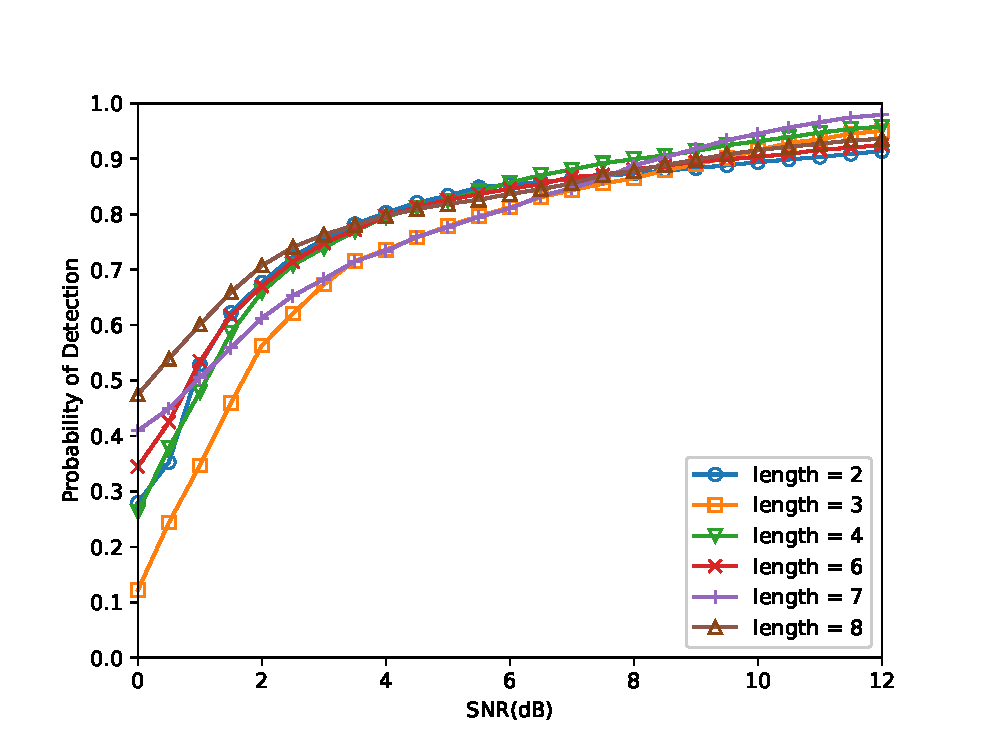
\includegraphics[scale=0.35]{result-length-conv.eps}}
	}
	\vspace{-1mm}
	\centerline{
		\subfigure{
			\rotatebox{90}{\scriptsize{~~~~~~~~~~~~~~~~~~~\textbf{(b) LDPC}}}
			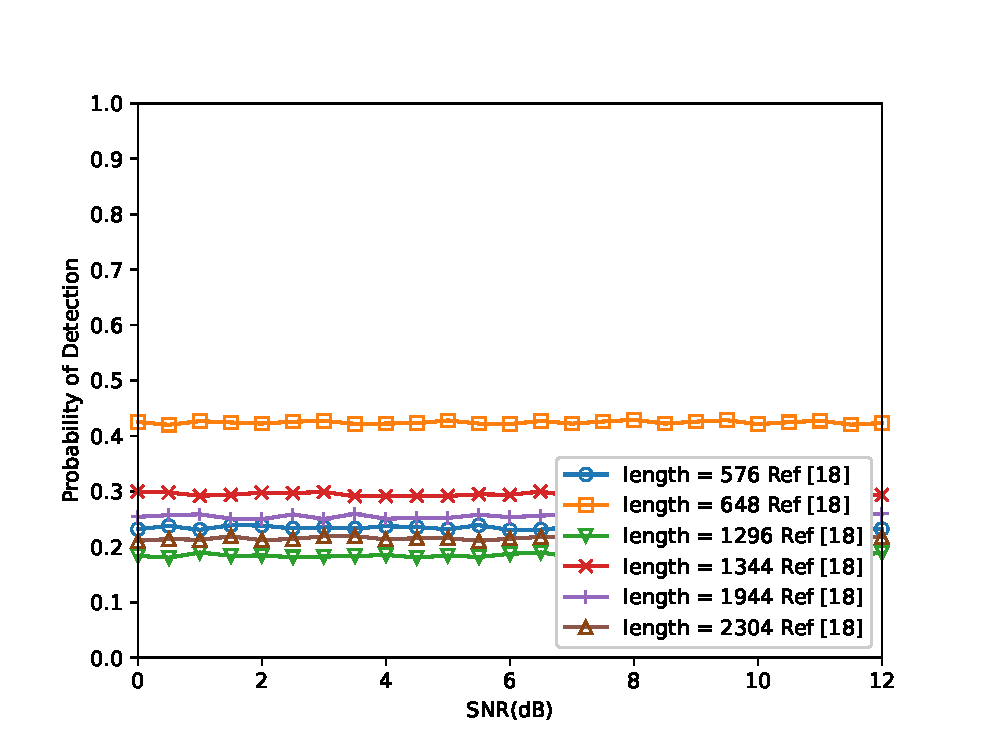
\includegraphics[scale=0.35]{result-length-ldpc-ncd.eps}
		}
		\subfigure{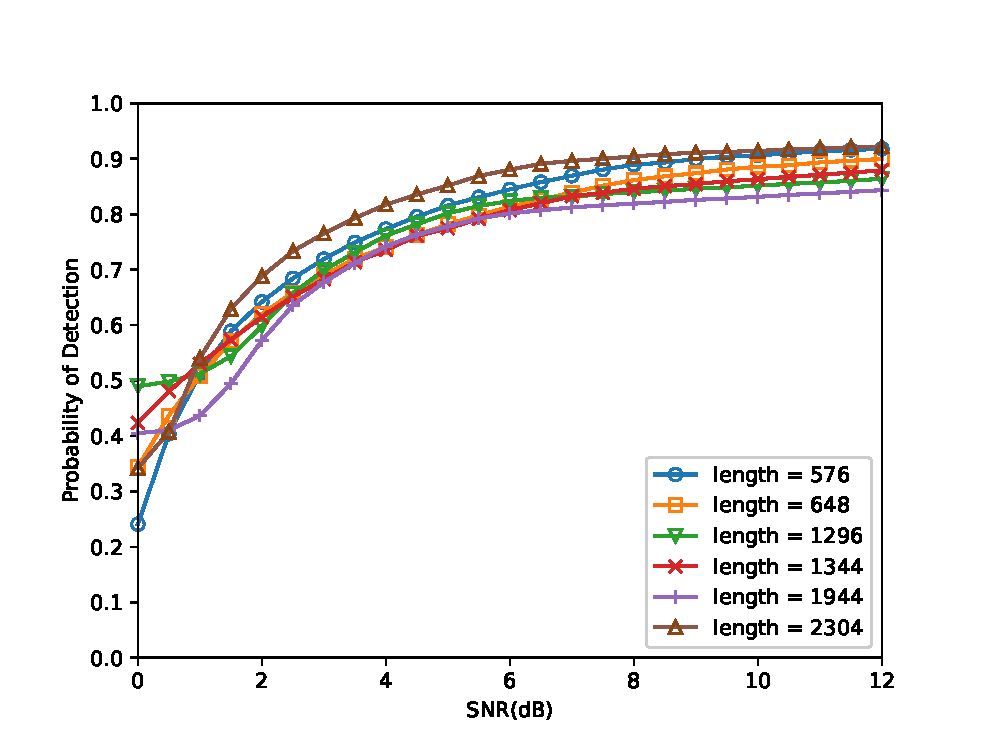
\includegraphics[scale=0.35]{result-length-ldpc-5.eps}}
		\subfigure{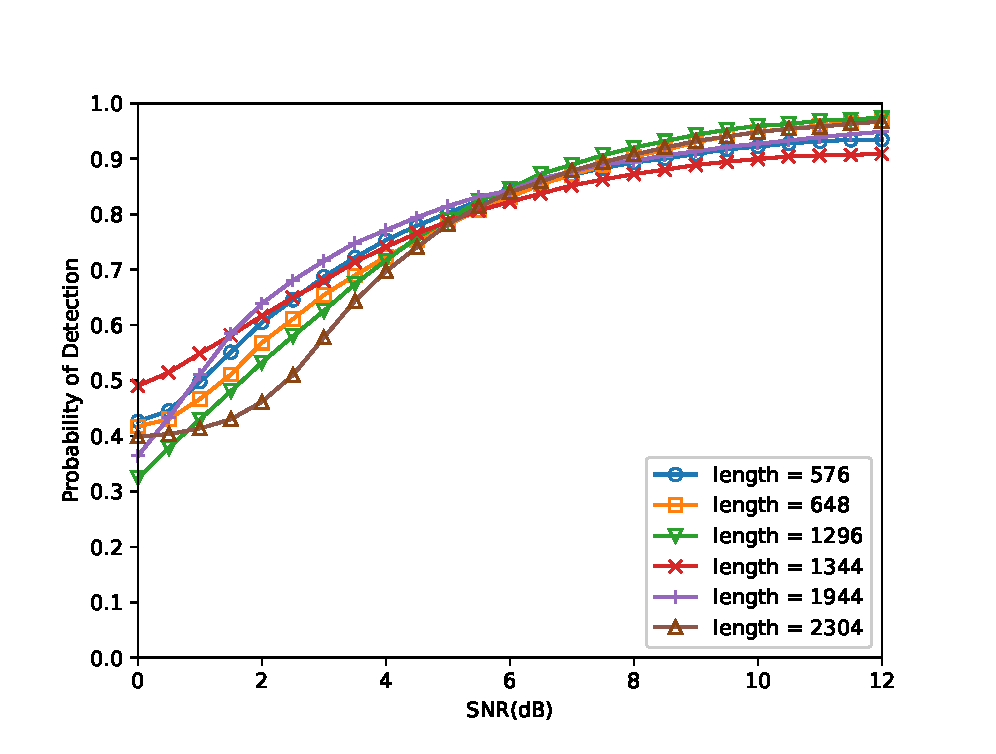
\includegraphics[scale=0.35]{result-length-ldpc.eps}}
	}
	\caption{Probability of detection for different coding lengths of (a) RCPC codes, (b) LDPC codes, by (1) NCD algorithm, (2) 5-dimensional feature, (3) 6-dimensional feature including GFFT, at different SNR ranges, the NCD algorithm is from \cite{bonvard2018classification}.}
	\label{fig}
\end{figure*}


\subsection{Coding Type Recognition}
We choose Bose-Chaudhuri-Hocquenghem (BCH) code, Reed-Solomon (RS) code, convolutional code, low-density parity-check (LDPC) code, turbo code, and polar code in the candidate set. In other words, we set the parameters of coding types as
\begin{equation}
	\mathcal{T} = \{bch, rs, conv, ldpc, turbo, polar\},
\end{equation}
these coding types are all widely used in wireless communication and satellite communication. The goal of coding type recognition in our experiment is not just concerned with identifying a particular type of all the codewords, but regard it as a multi-classification problem, identifying the corresponding types of all the codewords.

We assess the proposed recognizer for blind recognition veracity in experiments, Fig. 4 demonstrate the experimental results. As the figures show, the proposed recognizer could achieve good identification performance for BCH, RS, and polar codes in a wide range of SNR. To be specific, this recognizer can approximate 70\% for each channel code when SNR is not lower than 10dB, at this moment, it can effectively distinguish all channel coding types. We can find that the probability of detection for BCH codes and polar codes is very high, this is because BCH code is a relatively simple cyclic code, there is a close relationship between the generator polynomial and the minimum coding distance, and the coding theory of polar code is based on channel polarization theory, it is different significantly from other coding types.

For analyzing the misjudgment relationship between different channel coding types, when SNR = 10dB, the confusion matrix for blind recognition of coding types are shown in Fig. 5. The vertical axis is the actual label of the codeword, the horizontal axis is the recognition result bt the proposed recognizer, and the diagonal is the categories that are identified accurately. It indicates that the recognition accuracy all reaches 65\% for different channel coding types at SNR 10dB, and it can fully recognize BCH code and Polar code. It could be seen from the above results that there is relatively large confusion between RS code and LDPC code.

\begin{figure*}[tbp]
	\centerline{
		\rotatebox{0}{\scriptsize{
				~~~~~~~~~~~~
				\textbf{(1) contrast recognizer}
				~~~~~~~~~~~~~~~~~~~~~~~~~~~~~~~~}}
		\rotatebox{0}{\scriptsize{
				~~~~~~~~
				\textbf{(2) 5-dimensional}
				~~~~~~~~~~~~~~~~~~~~~~~~~~~~~~~~~~~~~~~~~~~}}
		\rotatebox{0}{\scriptsize{
				\textbf{(3) 6-dimensional}
				~~~~~~~~~~~~}}
	}
	\centerline{
		\subfigure{
			\rotatebox{90}{\scriptsize{~~~~~~~~~~~~~~~~~~~\textbf{(a) RCPC}}}
			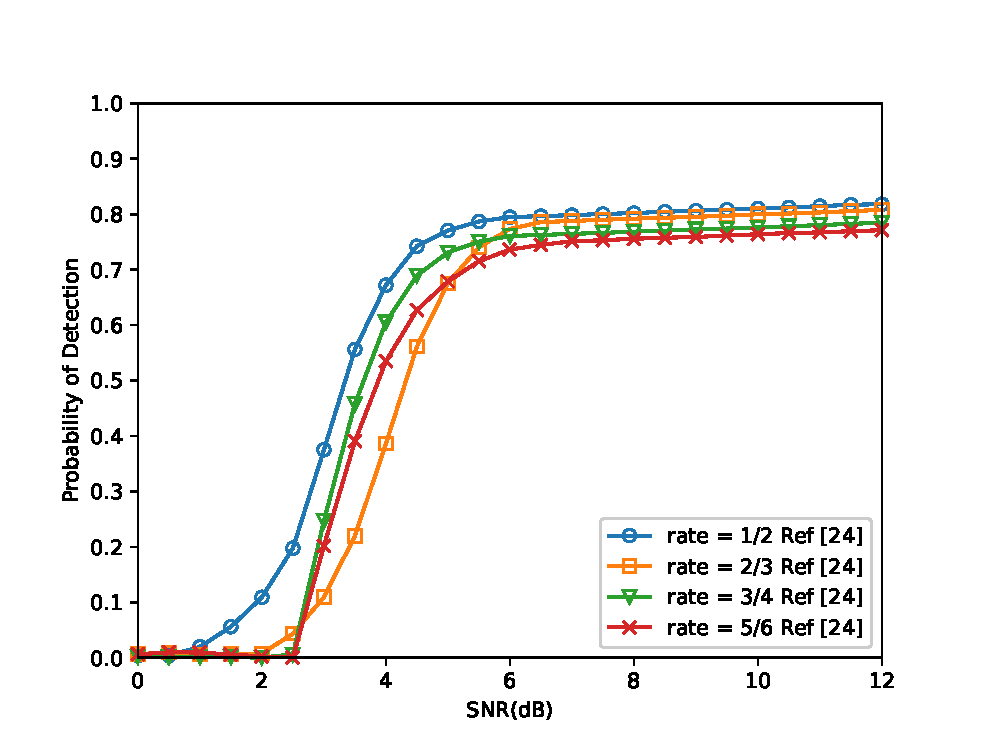
\includegraphics[scale=0.35]{result-rate-conv-ncd.eps}
		}
		\subfigure{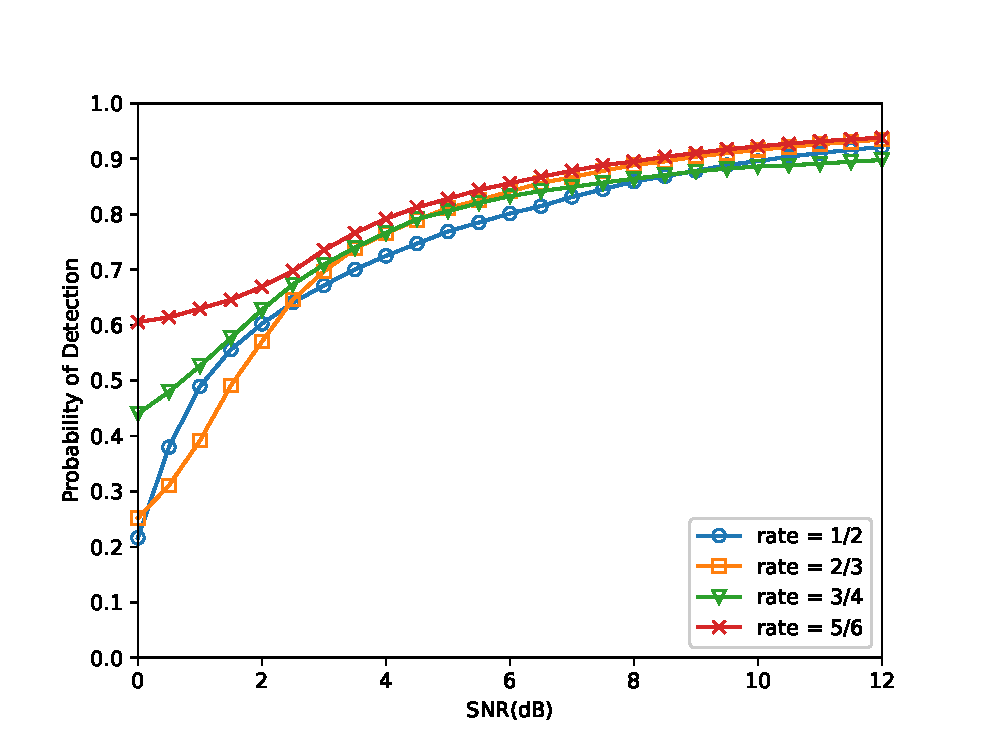
\includegraphics[scale=0.35]{result-rate-conv-5.eps}}
		\subfigure{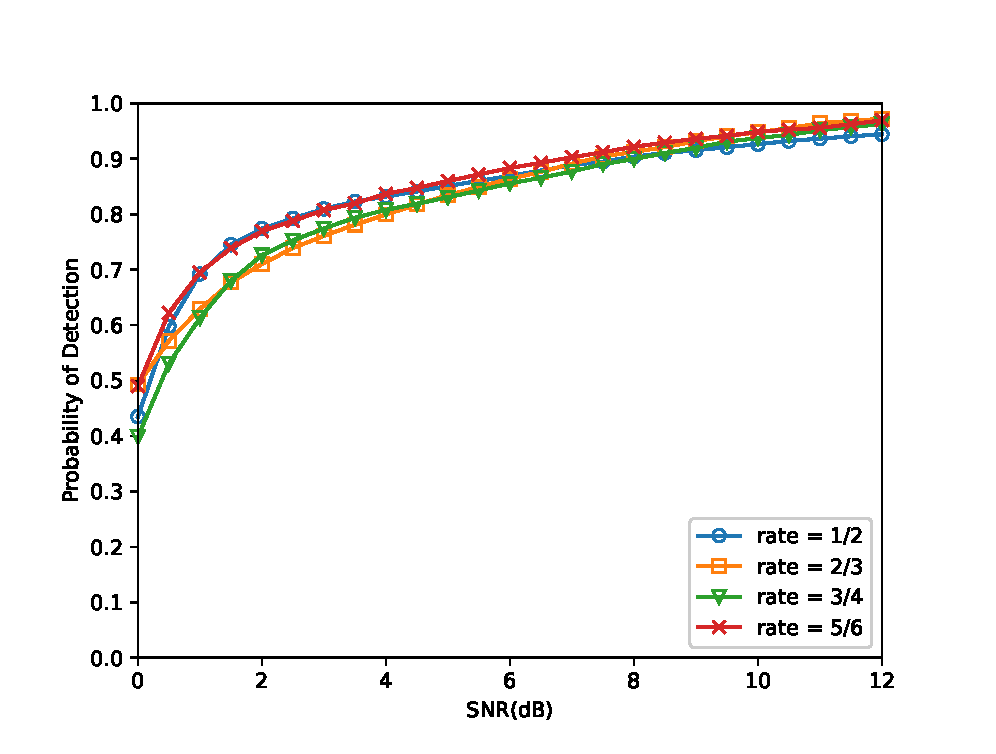
\includegraphics[scale=0.35]{result-rate-conv.eps}}
	}
	\vspace{-1mm}
	\centerline{
		\subfigure{
			\rotatebox{90}{\scriptsize{~~~~~~~~~~~~~~~~~~~\textbf{(b) LDPC}}}
			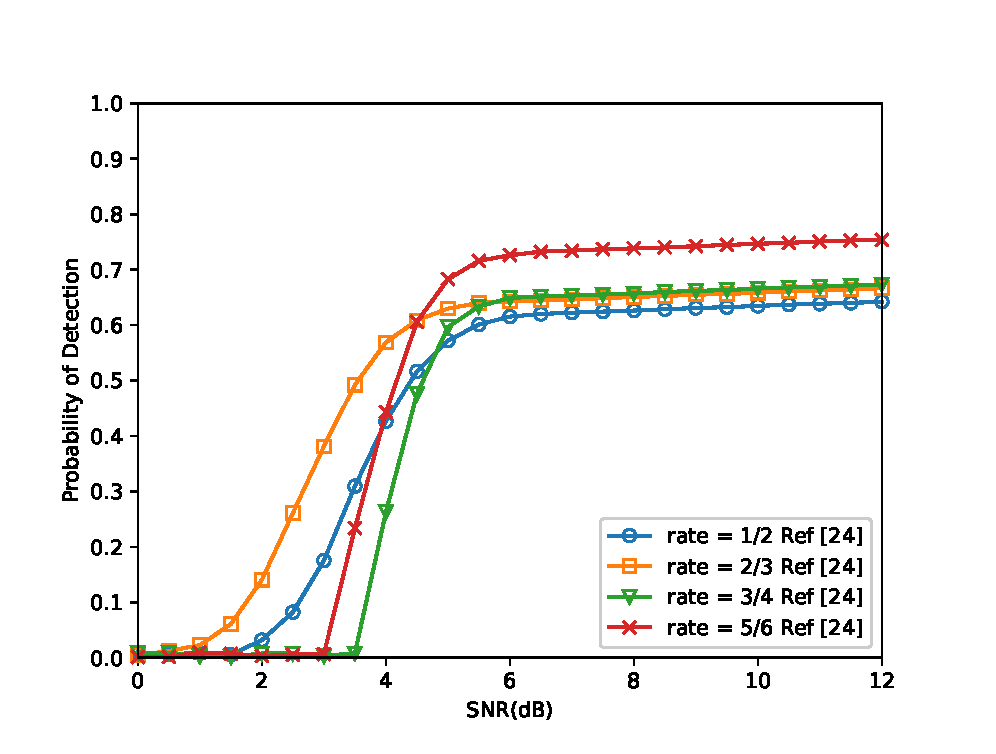
\includegraphics[scale=0.35]{result-rate-ldpc-ncd.eps}
		}
		\subfigure{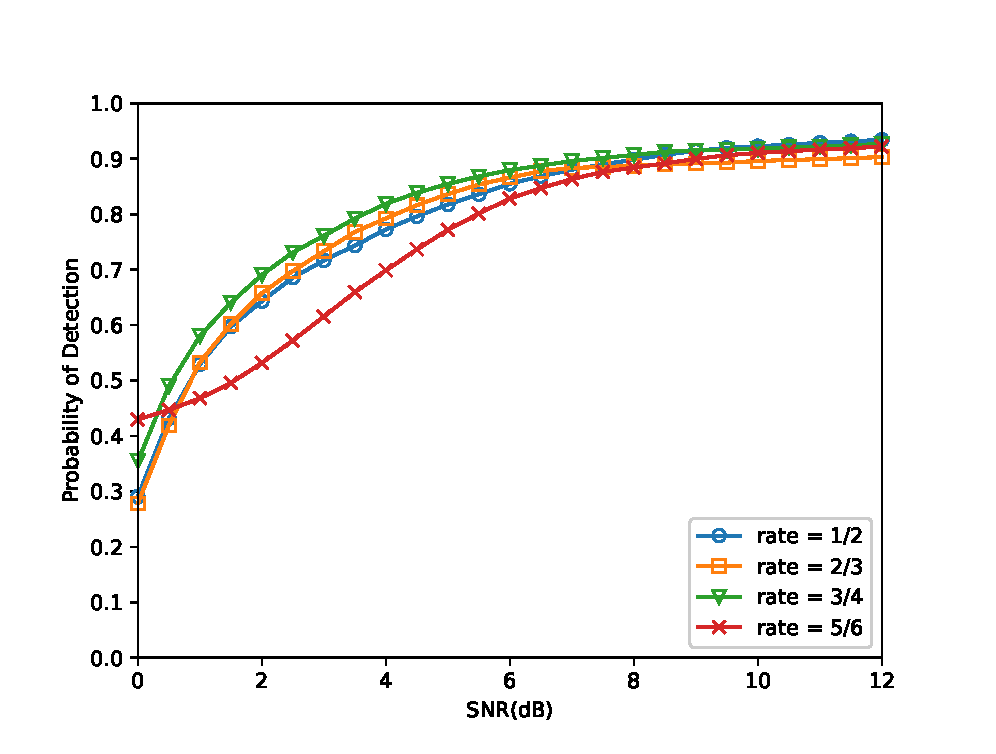
\includegraphics[scale=0.35]{result-rate-ldpc-5.eps}}
		\subfigure{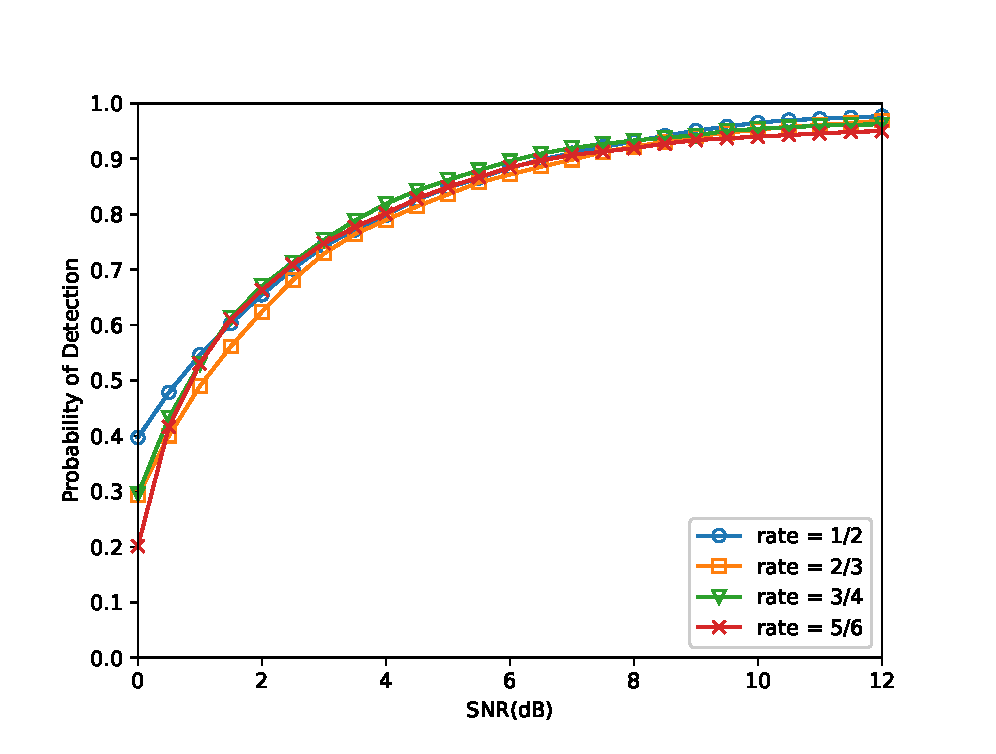
\includegraphics[scale=0.35]{result-rate-ldpc.eps}}
	}
	\caption{Probability of detection for different coding rates of (a) RCPC codes, (b) LDPC codes, by (1) contrast recognizer, (2) 5-dimensional feature, (3) 6-dimensional feature including GFFT, at different SNR ranges, the contrast recognizer is from \cite{shen2021blind}.}
	\label{fig}
\end{figure*}

\subsection{Coding Length Recognition}
The coding length is the length of the output codeword from the encoder, the coding rate is the quotient of the information bit length and the coding length, it also reflects the constraint relation between the information bit and the check bit in the codeword. In the total blindness environment, the feature of coding length is more evident than the coding rate. Therefore, we consider the recognition of the coding length at first, and then consider the coding rate.

We select rate-compatible punctured convolutional  (RCPC) codes and LDPC codes in coding length and rate recognition experiments, and there are 6 coding lengths in the candidate set for each channel code. For RCPC codes, we set the parameters of coding lengths as
\begin{equation}
	\mathcal{L} = \{2, 3, 4, 6, 7, 8\},
\end{equation}
and the generator polynomials $\mathcal{G}$ are from the DVB-RCS criterion \cite{Interaction2009}. Analogically, for LDPC codes, we set the parameters of coding lengths as
\begin{equation}
	\mathcal{L} = \{576, 648, 1296, 1344, 1944, 2304\},
\end{equation}
the parity-check matrixes $\mathcal{G}$ are from IEEE 802.11 criterion \cite{IEEE2012802} and  IEEE 802.16 criterion \cite{IEEE2013802}. At the same time, considering the computation complexity of GFFT is relatively more significant than other dimensional features, we compare 5-dimensional features without GFFT and 6-dimensional features including GFFT. In addition, the number of classes deficiency (NCD) algorithm of previous work \cite{bonvard2018classification} is also being compared.

To demonstrate the performance of our recognizer, we take simulation experiments, and Fig. 6 illustrates the results. Fig. 6(a) is the probability of detection for RCPC coding lengths, and Fig. 6(b) is the probability of detection for LDPC coding lengths. In Fig. 6(2) and Fig. 6(3), we can find that the boost of SNR advances recognition precision, especially recognition precision that reaches above 70\% when SNR is more significant than 4dB, the probability of detection for coding length is much improved. Meanwhile, the result of identification by the NCD algorithm is shown in Fig. 6(1), it could be seen that although the previous work is not affected by SNR, the performance is relatively lower than the proposed recognizer in this paper, the recognition accuracy is only about 20\%, which is significantly lower than our recognizer. 

In addition, comparing the 5-dimensional features without GFFT to the 6-dimensional features including GFFT, it shows that the 6-dimensional features are approximately 5\% better than 5-dimensional features when SNR is comparatively high. Therefore, although GFFT increases computational complexity, it can improve the recognition accuracy to a certain extent, and can be selected according to requirements in practical application. The results of simulation experiments testify to the effectiveness of the proposed recognizer for blind identification of coding length.


\subsection{Coding Rate Recognition}
Next, we evaluate the performance of the proposed recognizer in coding rate recognition, and compare it with the NCD algorithm. In experiments, the channel codes selected are the same as in the previous subsection. For RCPC codes and LDPC codes, we set the parameters of coding rates as
\begin{equation}
	\mathcal{R} = \left\{\frac{1}{2}, \frac{2}{3}, \frac{3}{4}, \frac{4}{5}\right\},
\end{equation}
the generator polynomials $\mathcal{G}$ of RCPC codes are also from the DVB-RCS criterion, and the parity-check matrixes $\mathcal{G}$ are also from IEEE 802.11 criterion and  IEEE 802.16 criterion. Similar to the last subsection, we compare 5-dimensional features without GFFT and 6-dimensional features including GFFT. In addition, we also select the contrast recognizer of previous work \cite{bonvard2018classification} to proceed with performance comparison.

Meanwhile, to illustrate the performance of this recognizer, the experiment results are shown in Fig. 7. Thereinto, Fig. 7(a) shows the probability of detection for RCPC coding rates, and Fig. 6(b) shows the probability of detection for LDPC coding rates. In Fig. 7(2) and Fig. 7(3), we can find that the identification accuracy exceeds 70\% when SNR is not lower than 5dB, the proposed recognizer can effectively distinguish the coding rate at the moment. As shown in Fig. 7(1), the recognition precision of the contrast recognizer is a little lower than our recognizer. The recognition is about 10\% lower than our recognizer when the SNR is greater than 9db, and about 20\% lower when the SNR is less than 9db.

Similarly, when SNR is comparatively high, the 6-dimensional features without GFFT are close to 5\% better than 5-dimensional features including GFFT, computational complexity and identification accuracy can be tradeoffs in a real environment. The above experimental results prove that the proposed channel coding recognizer in this paper can effectively distinguish different coding rates. 

\section{Conclusion}
This paper illustrates the feasibility of deep learning based channel coding recognition. This approach avoids manual feature extraction, which needs experience and professional skill of the handlers, meanwhile enormously reducing computation complexity. A multi-dimensional feature extraction method based on data randomness detection was proposed to extract the features of the received codewords. In addition, a novel ECA-Net based channel coding recognizer was presented, it shows a predominant property in the identification of coding types, coding length, and coding rates, simultaneously, this recognizer also has a decent generalization ability.

\bibliographystyle{IEEEtran} 
\bibliography{paper-ref}

\end{document}
